\documentclass[border=8pt]{standalone}
\usepackage{tikz}
\usetikzlibrary{arrows.meta,positioning,calc,fit}
\begin{document}
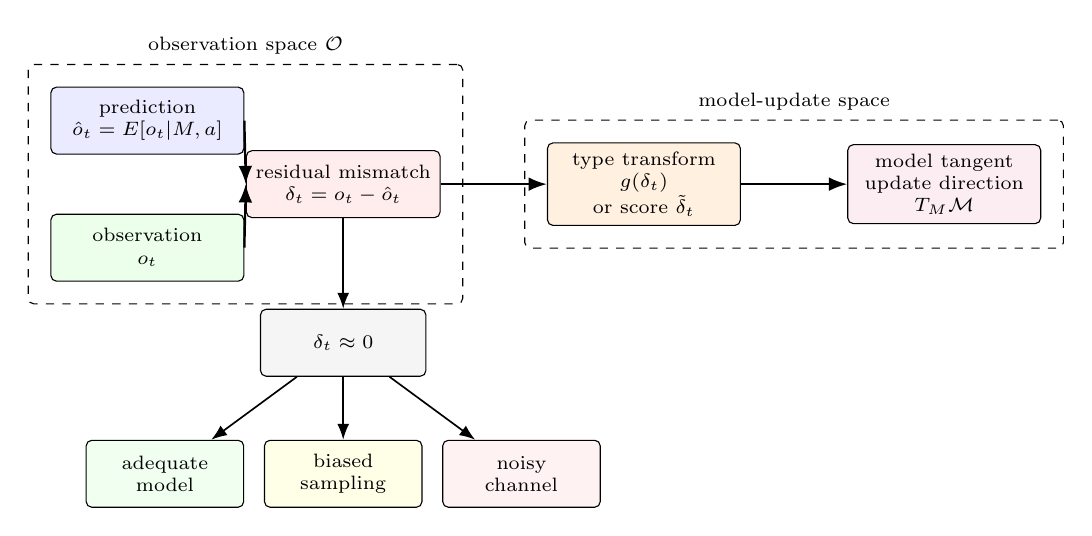
\begin{tikzpicture}[
  box/.style={draw, rounded corners=2pt, align=center, minimum width=2.45cm, minimum height=0.85cm, font=\scriptsize},
  space/.style={draw, rounded corners=2pt, dashed, inner sep=8pt},
  transform/.style={draw, rounded corners=2pt, align=center, minimum width=2.45cm, minimum height=0.9cm, font=\scriptsize, fill=orange!12},
  note/.style={align=center, font=\scriptsize},
  arr/.style={-Latex, thick},
  thinarr/.style={-Latex, semithick}
]

\node[box, fill=blue!8] (pred) {prediction\\$\hat o_t=E[o_t|M,a]$};
\node[box, fill=green!8, below=0.75cm of pred] (obs) {observation\\$o_t$};
\node[box, fill=red!7, right=1.25cm of $(pred)!0.5!(obs)$] (delta) {residual mismatch\\$\delta_t=o_t-\hat o_t$};

\draw[arr] (pred.east) -- (delta.west);
\draw[arr] (obs.east) -- (delta.west);

\node[transform, right=1.35cm of delta] (g) {type transform\\$g(\delta_t)$\\or score $\tilde\delta_t$};
\node[box, fill=purple!7, right=1.35cm of g] (tan) {model tangent\\update direction\\$T_M\mathcal M$};
\draw[arr] (delta) -- (g);
\draw[arr] (g) -- (tan);

\node[space, fit=(pred)(obs)(delta), label={[font=\scriptsize]above:observation space $\mathcal O$}] {};
\node[space, fit=(g)(tan), label={[font=\scriptsize]above:model-update space}] {};

\node[box, fill=gray!8, below=1.15cm of delta, minimum width=2.1cm] (zero) {$\delta_t\approx 0$};
\node[box, fill=green!6, below left=0.8cm and 0.2cm of zero, minimum width=2.0cm] (fit) {adequate\\model};
\node[box, fill=yellow!10, below=0.8cm of zero, minimum width=2.0cm] (bias) {biased\\sampling};
\node[box, fill=red!5, below right=0.8cm and 0.2cm of zero, minimum width=2.0cm] (noise) {noisy\\channel};
\draw[thinarr] (delta) -- (zero);
\draw[thinarr] (zero) -- (fit);
\draw[thinarr] (zero) -- (bias);
\draw[thinarr] (zero) -- (noise);

\end{tikzpicture}
\end{document}
